% Copyright 2004 by Till Tantau <tantau@users.sourceforge.net>.
%
% In principle, this file can be redistributed and/or modified under
% the terms of the GNU Public License, version 2.
%
% However, this file is supposed to be a template to be modified
% for your own needs. For this reason, if you use this file as a
% template and not specifically distribute it as part of a another
% package/program, I grant the extra permission to freely copy and
% modify this file as you see fit and even to delete this copyright
% notice. 

\documentclass{beamer}
% Replace the \documentclass declaration above
% with the following two lines to typeset your 
% lecture notes as a handout:
%\documentclass{article}
%\usepackage{beamerarticle}

\usepackage{amsmath}
\usepackage{amssymb}
\usepackage{bm}
\usepackage{mathrsfs}
\usepackage{bclogo}

\newcommand{\Probe}[1]{\mathbb{P}\left({#1}\right)}
\newcommand{\Prob}[1]{\mathbb{P}\left\{ {#1} \right\}}
\newcommand{\Expect}{\operatorname{\mathbb{E}}}
\newcommand{\Var}{\operatorname{Var}}

\newcommand{\normal}{\textsc{normal}}
\newcommand{\erf}{\operatorname{erf}}
\newcommand{\norm}[1]{\left\Vert {#1} \right\Vert}
\newcommand{\normsq}[1]{\norm{#1}^2}



%%% Vector and matrix operators

\newcommand{\vct}[1]{\bm{#1}}
\newcommand{\mtx}[1]{\bm{#1}}
\DeclareMathOperator{\Ima}{Im}
%\newcommand{\mtx}[1]{\mathsf{#1}}
%\newcommand{\mtx}[1]{\mathsfsl{#1}}


\newcommand{\transp}{\mathrm{T}}
\newcommand{\adj}{*}
\newcommand{\psinv}{\dagger}
\newcommand{\anum}[1]{{\footnotesize{#1}\quad}}
\newcommand{\econst}{\mathrm{e}}
\newcommand{\Id}{\mathbf{I}}


% There are many different themes available for Beamer. A comprehensive
% list with examples is given here:
% http://deic.uab.es/~iblanes/beamer_gallery/index_by_theme.html
% You can uncomment the themes below if you would like to use a different
% one:
%\usetheme{AnnArbor}
%\usetheme{Antibes}
%\usetheme{Bergen}
%\usetheme{Berkeley}
%\usetheme{Berlin}
%\usetheme{Boadilla}
%\usetheme{boxes}
%\usetheme{CambridgeUS}
%\usetheme{Copenhagen}
%\usetheme{Darmstadt}
%\usetheme{default}
%\usetheme{Frankfurt}
% \usetheme{Goettingen}
%\usetheme{Hannover}
%\usetheme{Ilmenau}
%\usetheme{JuanLesPins}
%\usetheme{Luebeck}
\usetheme{Madrid}
%\usetheme{Malmoe}
%\usetheme{Marburg}
%\usetheme{Montpellier}
%\usetheme{PaloAlto}
%\usetheme{Pittsburgh}
%\usetheme{Rochester}
%\usetheme{Singapore}
%\usetheme{Szeged}
%\usetheme{Warsaw}

\title{Probabilistic Algorithms for Finding \\ Matrix Decompositions}

% A subtitle is optional and this may be deleted
\subtitle{Sparsity and Compressed Sensing \\ MVA 2017/18 - ENS Cachan}

\author{Alex Nowak}
% - Give the names in the same order as the appear in the paper.
% - Use the \inst{?} command only if the authors have different
%   affiliation.

% \institute[Universities of Somewhere and Elsewhere] % (optional, but mostly needed)
% {
%   \inst{1}%
%   Department of Computer Science\\
%   University of Somewhere
%   \and
%   \inst{2}%
%   Department of Theoretical Philosophy\\
%   University of Elsewhere}
% - Use the \inst command only if there are several affiliations.
% - Keep it simple, no one is interested in your street address.

\date{Advised by: Gabriel Peyr\'e}
% - Either use conference name or its abbreviation.
% - Not really informative to the audience, more for people (including
%   yourself) who are reading the slides online

\subject{Theoretical Computer Science}
% This is only inserted into the PDF information catalog. Can be left
% out. 

% If you have a file called "university-logo-filename.xxx", where xxx
% is a graphic format that can be processed by latex or pdflatex,
% resp., then you can add a logo as follows:

% \pgfdeclareimage[height=0.5cm]{university-logo}{university-logo-filename}
% \logo{\pgfuseimage{university-logo}}

% Delete this, if you do not want the table of contents to pop up at
% the beginning of each subsection:
\AtBeginSubsection[]
{
  \begin{frame}<beamer>{Outline}
    \tableofcontents[currentsection,currentsubsection]
  \end{frame}
}

% Let's get started
\begin{document}

\begin{frame}
  \titlepage
\end{frame}

% \begin{frame}{Outline}
%   \tableofcontents
%   % You might wish to add the option [pausesections]
% \end{frame}

% Section and subsections will appear in the presentation overview
% and table of contents.
\section{Presentation of the Problem}

\begin{frame}{Problem: Low rank approximation of a matrix}
  $$\begin{array}{ccccccccccc}
    \mtx{A} &\approx& \mtx{B} & \mtx{C},\\
    m\times n && m \times k & k\times n.
    \end{array}$$
  \begin{itemize}
  \item {
    \textbf{Standard Decompositions:}
    \begin{enumerate}
      \item SVD: $$\mtx{A}=\left(\mtx{U}\mtx{\Sigma}^{1/2}\right)\left(\mtx{V}\mtx{\Sigma}^{1/2}\right)^\adj$$
      \item QR: $$\mtx{A}=\mtx{Q}\mtx{R}$$
    \end{enumerate}
  }
  \item {
    \textbf{Classical Algorithms:}
    \begin{enumerate}
      \item Computationally expensive: $\mathcal{O}(mnk)$.
      \item Need $\mathcal{O}(k)$ passes over data.
      \item Can't deal with inaccurate matrices.
    \end{enumerate}
  }
  \end{itemize}
  $$ \implies \text{Not adequate to deal with massive datasets!} $$
\end{frame}

\section{Algorithm}

\begin{frame}{Two Stages Solution}
\begin{itemize}
  \item \textbf{Stage A:} (\textit{Randomized}) Find $m\times k$ orthonormal $\mtx{Q}$ whose columns approximate the 
  range of $\mtx{A}$:
  $$ \mtx{A} \approx \mtx{Q}\mtx{Q}^\adj\mtx{A} $$
  \item \textbf{Stage B:} (\textit{Deterministic}) Use $\mtx{Q}$ to find the desired
  decomposition. E.g, set $\mtx{B}=\mtx{Q}$ and $\mtx{C}=\mtx{Q}^\adj\mtx{A}$
\end{itemize}
\end{frame}

\begin{frame}{Stage A: Randomize!}
\begin{figure}[ht]
\begin{center}
\fbox{
\begin{minipage}{.9\textwidth}
\begin{center}
\textsc{Randomized Range Finder}
\end{center}
\begin{tabbing}
\hspace{5mm} \= \hspace{5mm} \= \hspace{5mm} \= \hspace{5mm} \= \kill
\anum{1} \>Draw an $n\times \ell$ Gaussian random matrix $\mtx{\Omega}$.\\
\anum{2} \>Form the $m\times \ell$ matrix $\mtx{Y} = \mtx{A}\mtx{\Omega}$.\\
\anum{3} \>Construct an $m \times \ell$ matrix $\mtx{Q}$ whose columns form an orthonormal\\
         \> basis for the range of $\mtx{Y}$, e.g., using the QR factorization $\mtx{Y} = \mtx{Q}\mtx{R}$.
\end{tabbing}
\end{minipage}}
\end{center}
\end{figure}
\begin{itemize}
  \item If we set $\ell=k+p$ with $p>0$ ($p<<k$) the \textit{oversampling parameter},
  we can control the error $\| \mtx{A}-\mtx{Q}\mtx{Q}^\adj\mtx{A}\|$ with arbitrary
  precision! \bcsmbh
  $$
\Expect \norm{\mtx{A}-\mtx{Q}\mtx{Q}^\adj\mtx{A}}
    \leq \left(1 + \sqrt{\frac{k}{p-1}} \right) \sigma_{k+1}
        + \frac{\econst\sqrt{k+p}}{p}
        \left(\sum\nolimits_{j>k} \sigma_{j}^2 \right)^{1/2}.$$
  \item But, error large if singular values $(\sigma_i)_{i=1}^r$ decay slowly... \bcsmmh
  \item But, product $\mtx{A}\mtx{\Omega}$ too expensive... $\mathcal{O}(mn\ell)$ \hspace{0.5cm} \bcsmmh
\end{itemize}
\end{frame}

\begin{frame}{Stage A: Solving the two issues.}
\begin{itemize}
  \item If $\mtx{A}$ has slow decaying singular values $(\sigma_i)_{i=1}^r$, take powers!\bcsmbh
  $$ \mtx{Y}=\mtx{B}\mtx{\Omega}\hspace{0.5cm}\mtx{B}=(\mtx{A}\mtx{A}^\adj)^q\mtx{A} \hspace{0.5cm} \sigma_j(\mtx{B}) = \sigma_j(\mtx{A})^{2q+1},
      \hspace{0.5cm} j=1,2,3,\ldots$$
      $$ \frac{\Expect \norm{\mtx{A}-\mtx{Q}\mtx{Q}^\adj\mtx{A}}}{\sigma_{k+1}}
    \leq \left[ 1 + \sqrt{\frac{k}{p-1}}
    + \frac{\econst\sqrt{k+p}}{p} \cdot \sqrt{ \min\{m,n\} - k } \right]^{1/(2q+1)}
    . $$

  \item Make the product $\mtx{A}\mtx{\Omega}$ cheaper by using a 
  \textit{structured random matrix} instead of Gaussian. 

  Use \textit{Subsampled Random Fourier Transform}(SRFT)
  $$ \mtx{\Omega} = \sqrt{n/\ell} \cdot \mtx{DFR}^\adj $$
  Can compute the sample
matrix $\mtx{Y} = \mtx{A\Omega}$ in $\mathcal{O}(mn\log(\ell))$ operations via a
\textit{subsampled FFT}. \bcsmbh
\end{itemize}
\end{frame}

\begin{frame}{Stage B: Construct $\mtx{A}\approx\mtx{B}\mtx{C}$ decomposition from $\mtx{Q}$.}
\textbf{Obs:} Deterministic stage.
\begin{itemize}
  \item \textbf{Direct SVD:} Set $\mtx{B}=\mtx{Q}$ and $\mtx{C}=\mtx{Q}^\adj\mtx{A}$.
  $$ \implies \text{Product }\mtx{Q}^\adj\mtx{A}\text{ costs }
  \mathcal{O}(mnk)\text{, too expensive!} $$

  \item \textit{Solution}: Can be reduced to $\mathcal{O}(k^2(m+n))$
  via \textit{row extraction}, but an additive error term comes up.
\end{itemize}
\end{frame}

\section{Theoretical analysis}
\begin{frame}{Theory: Expectation and high probability error bounds.}
\textbf{Obs:} Deterministic stage.
\begin{itemize}
  \item \textbf{Expectation bound:}
  $$
\Expect \norm{\mtx{A}-\mtx{Q}\mtx{Q}^\adj\mtx{A}}
    \leq \left(1 + \sqrt{\frac{k}{p-1}} \right) \sigma_{k+1}
        + \frac{\econst\sqrt{k+p}}{p}
        \left(\sum\nolimits_{j>k} \sigma_{j}^2 \right)^{1/2}.$$

  with probability 
  \item \textbf{Tail bound:}
  $$
\norm{ (\Id - \mtx{P}_{\mtx{Y}}) \mtx{A} } \leq $$
    $$\leq \left( 1 + 8 \sqrt{(k + p) \cdot p \log p} \right) \sigma_{k+1}
        + 3 \sqrt{k+p} \left( \sum\nolimits_{j > k} \sigma_j^2 \right)^{1/2},
$$
with failure probability at most $6 p^{-p}$..

\textbf{Remark:} Very fast decay with \textit{oversampling parameter} $p$.
\end{itemize}
\end{frame}

\section{Experiments}
\begin{frame}{Experiment: Compare theoretical bound with numerical error
for powers of normalized gaussian matrices $\mtx{A}$.}
\begin{figure}[H]\label{fig:exp1-1}
\begin{center}
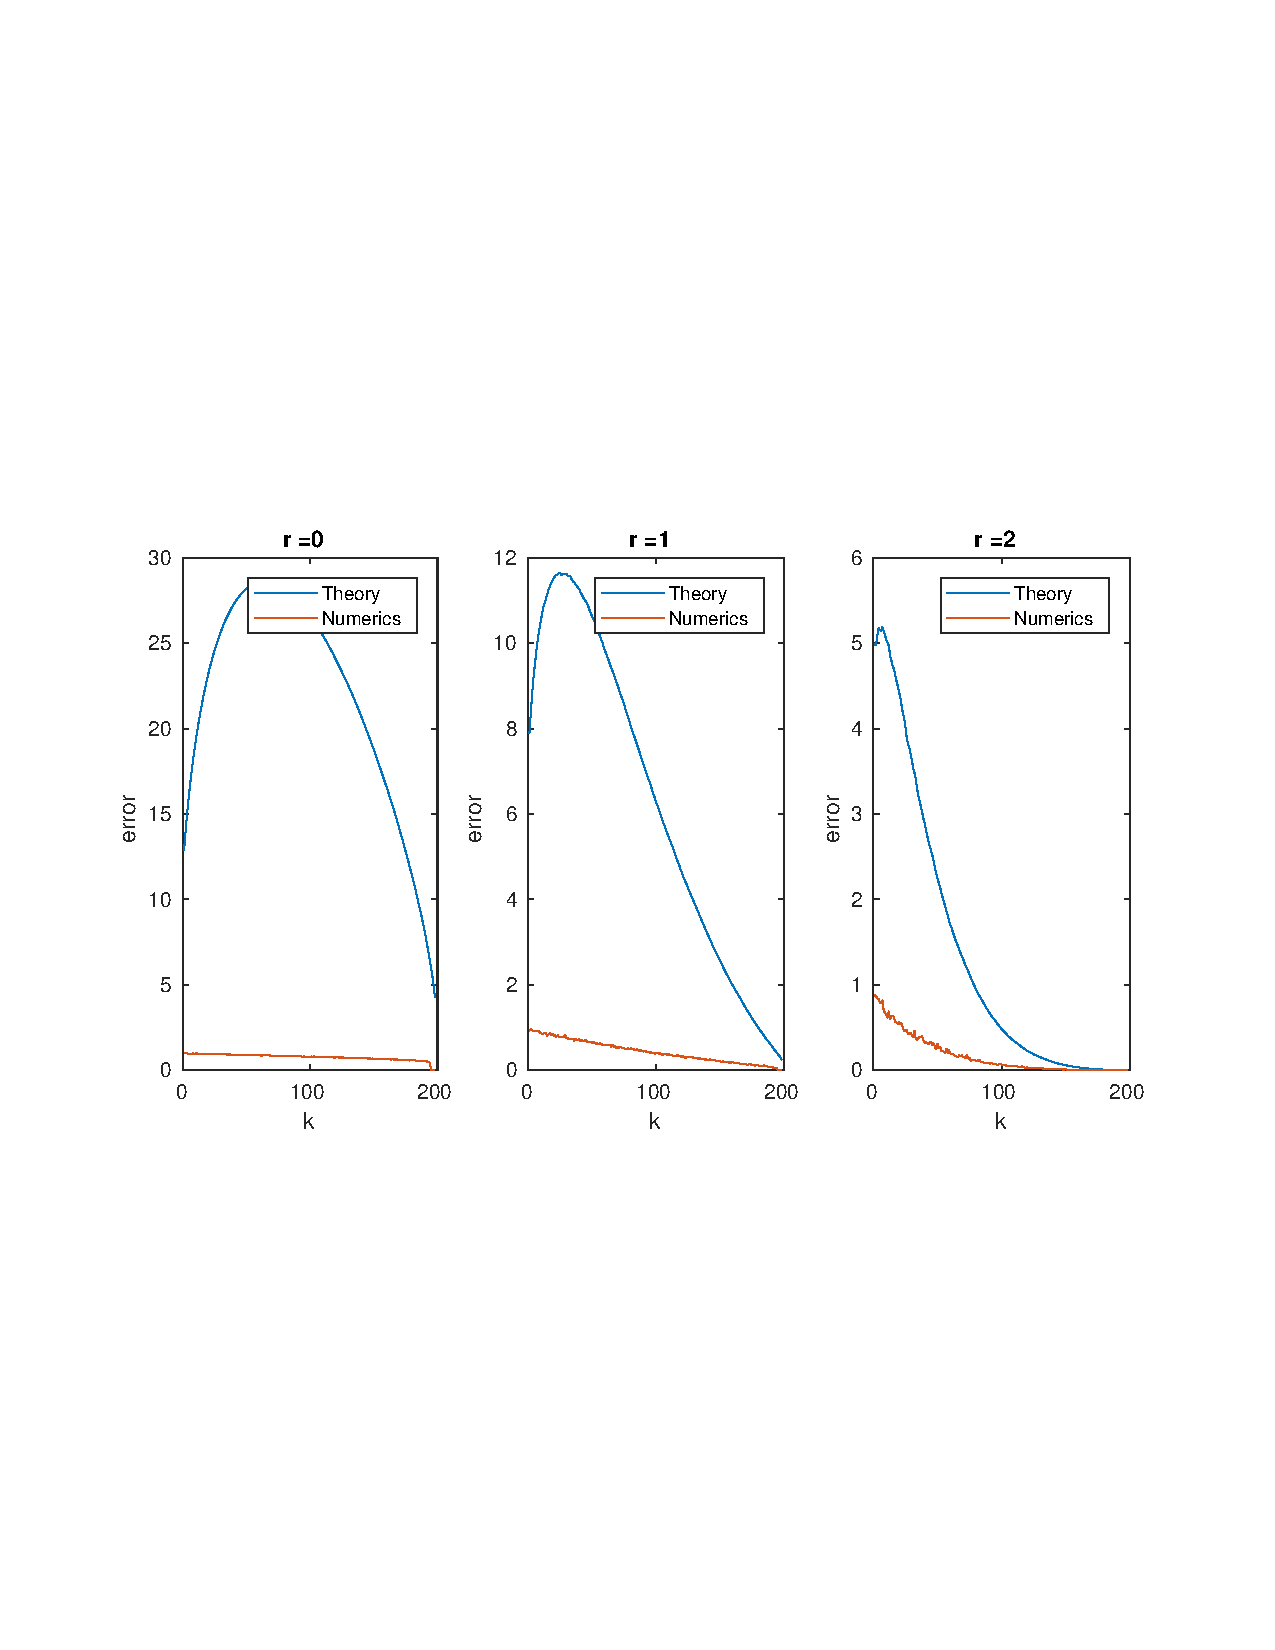
\includegraphics[width=0.8\textwidth, trim=0cm 8cm 0cm 9cm, clip=true]{../report/figures/1-4.pdf}
\end{center}
\caption{Comparison between theoretical mean bound
and numerical error produced by \textit{Randomized Range Finder}
 for $(\mtx{A}\mtx{A}^\adj)^r\mtx{A}$ with $r=0,1,2$. }
\end{figure}
\end{frame}

\begin{frame}{Experiment: Compare theoretical bound with numerical error
for powers of normalized gaussian matrices $\mtx{A}$.}
\begin{figure}[H] \label{fig:exp1-2}
\begin{center}
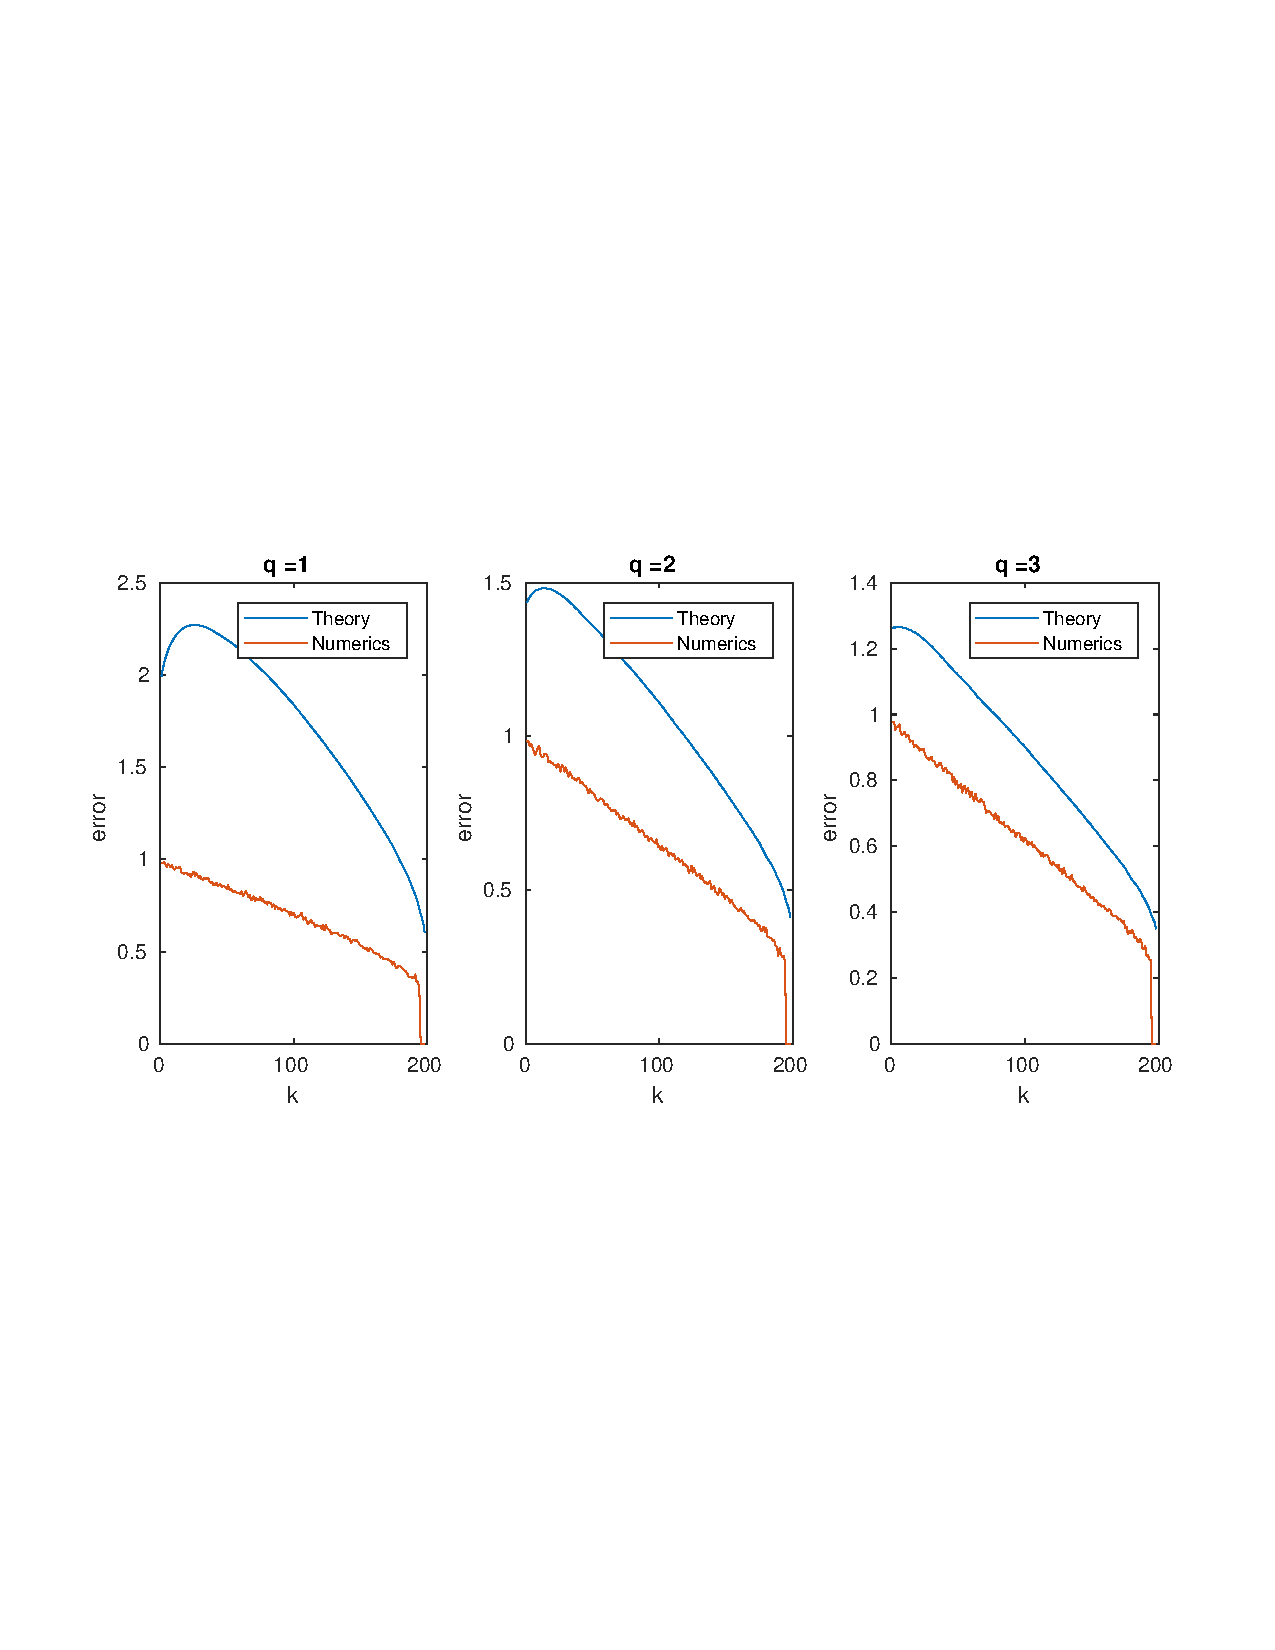
\includegraphics[width=0.8\textwidth, trim=0cm 8cm 0cm 9cm, clip=true]{../report/figures/1-5.pdf}
\end{center}
\caption{Comparison between theoretical mean bound
and numerical error produced by \textit{Randomized Power Iteration}
for $\mtx{A}$ and $q=1,2,3$}
\end{figure}
\end{frame}

\begin{frame}{Experiment: MNIST and Laplacian eigenvectors of image patches.}
\begin{figure}[H] \label{fig:exp2}
\begin{center}
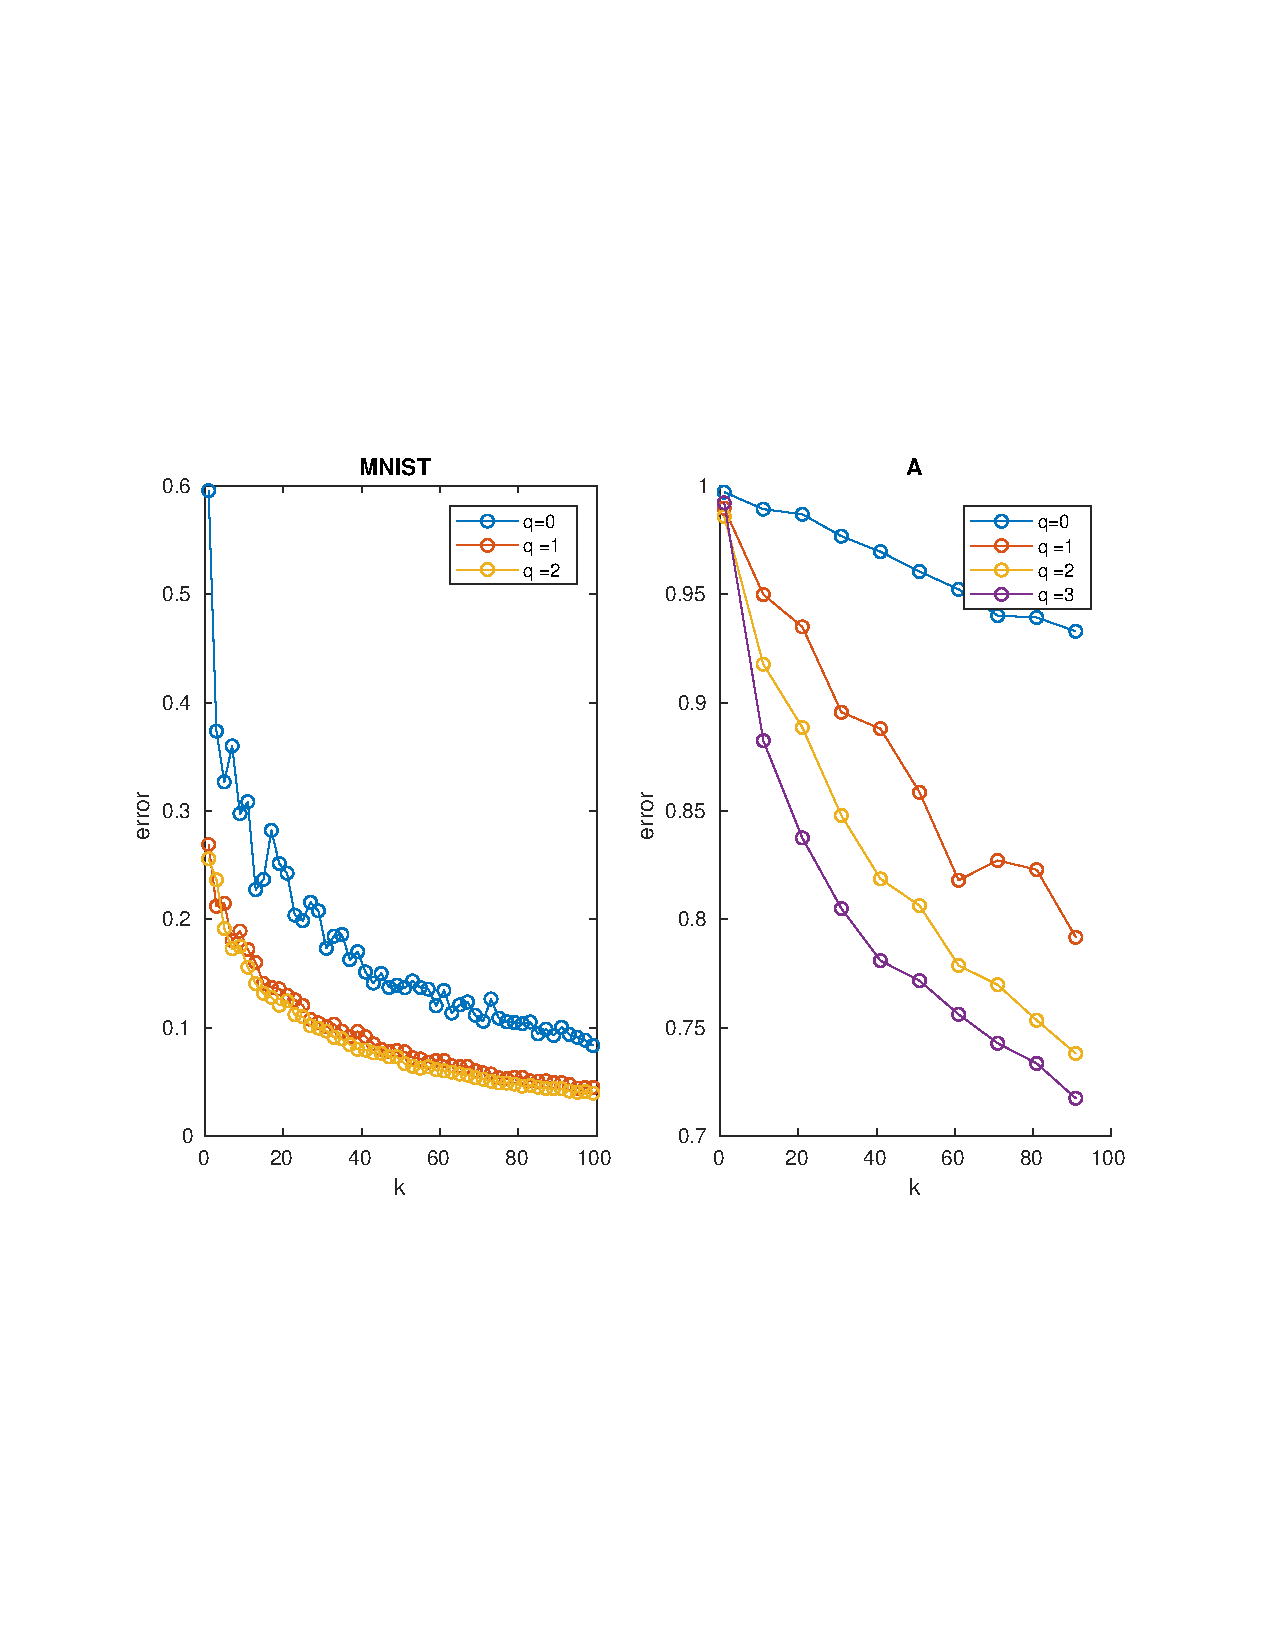
\includegraphics[width=0.8\textwidth, trim=0cm 8cm 0cm 7cm, clip=true]{../report/figures/2-1.pdf}
\end{center}
\caption{\textbf{Left:} Fast decaying singular values. \textbf{Right:} Slow decaying singular
values.}
\end{figure}
\end{frame}


\section{Take Away Message / Future directions / Critics}
\begin{frame}{Take Away Message / Future directions / Critics}
\begin{itemize}
  \item Necessary tool for Data Scientists working with massive or inaccurate 
  datasets.
  \item Methods with strong experimental evidence backed up with theory.
  \item Future directions: Improve error bounds sharpness under hypothesis
  of matrix $\mtx{A}$.
  \item 
\end{itemize}
\end{frame}

% All of the following is optional and typically not needed. 
% \appendix
% \section<presentation>*{\appendixname}
% \subsection<presentation>*{For Further Reading}

% \begin{frame}[allowframebreaks]
%   \frametitle<presentation>{For Further Reading}
    
%   \begin{thebibliography}{10}
    
%   \beamertemplatebookbibitems
%   % Start with overview books.

%   \bibitem{Author1990}
%     A.~Author.
%     \newblock {\em Handbook of Everything}.
%     \newblock Some Press, 1990.
 
    
%   \beamertemplatearticlebibitems
%   % Followed by interesting articles. Keep the list short. 

%   \bibitem{Someone2000}
%     S.~Someone.
%     \newblock On this and that.
%     \newblock {\em Journal of This and That}, 2(1):50--100,
%     2000.
%   \end{thebibliography}
% \end{frame}

\end{document}


